\section{Наблюдаемое подпространство}

Рассмотрим систему: 
\begin{equation}
    \begin{cases}
        \dot{x} = Ax \\
        y = Cx,
    \end{cases}
\end{equation}
где 
\begin{equation}
    \begin{array}{cc}
        A = \begin{bmatrix}
            -10 & -7 & -18 \\
            -3 & -4 & -8 \\
            8 & 2 & 11
        \end{bmatrix}, &
        C = \begin{bmatrix}
            0 & -1 & -1
        \end{bmatrix}
    \end{array}
\end{equation}

\subsection{Наблюдаемость системы}
\subsubsection{Матрица наблюдаемости}
\begin{equation}
    W = \begin{bmatrix}
        0  & -1  & -1 \\ 
        -5  & 2  & -3 \\ 
        20  & 21  & 41 \\ 
        \end{bmatrix}
\end{equation}
Определим ранг матрицы наблюдаемости:
\begin{equation}
    \text{rank}(W) = 2
\end{equation}
Так как ранг матрицы наблюдаемости меньше порядка системы, то система не является полностью наблюдаемой. 

\subsubsection{Наблюдаемость собственных значений}
Для каждого собственного значения найдем матрицу Хаутуса $H_i = [A - \lambda_i, C]^T$:
\begin{enumerate}
    \item $\lambda_1 = -2 + 5j: \begin{bmatrix}
        -8 - 5j  & -7  & -18 \\ 
        -3  & -2 - 5j  & -8 \\ 
        8  & 2  & 13 - 5j \\ 
        0  & -1  & -1 \\ 
        \end{bmatrix} $, $\text{rank}(H_1) = 3$, собственное значение наблюдаемо

    \item $\lambda_2 = -2 - 5j: \begin{bmatrix}
        -8 + 5j  & -7  & -18 \\ 
        -3  & -2 + 5j  & -8 \\ 
        8  & 2  & 13 + 5j \\ 
        0  & -1  & -1 \\ 
    \end{bmatrix}$, $\text{rank}(H_2) = 3$, собственное значение наблюдаемо

    \item $\lambda_3 = 1: \begin{bmatrix}
        -11  & -7  & -18 \\ 
        -3  & -5  & -8 \\ 
        8  & 2  & 10 \\ 
        0  & -1  & -1 \\ 
    \end{bmatrix}$, $\text{rank}(H_3) = 2$, собственное значение не наблюдаемо
    
\end{enumerate}

Как и было показано ранее, система не является полностью наблюдаемой. Таким образом, наблюдаемое подпространство системы состоит из двух векторов.

\subsubsection{Диагональная форма системы}
Диагональная форма системы:
\begin{equation}
    \begin{cases}
        \dot{\hat{x}} = \begin{bmatrix}
            1 & 0 & 0 \\
            0 & -2-5j & 0 \\
            0 & 0 & -2+5j
        \end{bmatrix} \hat{x} \\ 
        y = \begin{bmatrix}
            0 & -0.5+0.5j & -0.5-0.5j
        \end{bmatrix} \hat{x}
    \end{cases}
\end{equation}

Первый элемент вектора $CP$ равен нулю, откуда можно сделать вывод, что первая мода системы не является наблюдаемой. 

\subsection{Грамиан наблюдаемости}
Найдем грамиан наблюдаемости $Q(3)$:
\begin{equation}
    Q(3) = \begin{bmatrix}
        0.11  & 0.04  & 0.15 \\ 
        0.04  & 0.14  & 0.19 \\ 
        0.15  & 0.19  & 0.34 \\ 
        \end{bmatrix}
\end{equation}
Собственные числа грамиана наблюдаемости:
\begin{equation}
    \sigma(Q(3)) = \{0, 0.083, 0.51\}
\end{equation}
Есть одно нулевое собственное число, что говорит о том, что система не является полностью наблюдаемой.

\subsection{Наблюдение системы}
Будем считать, что выход системы соответствует функции $y(t)$:
\begin{equation}
    y(t) = e^{-2t} \cos(5t) -2e^{-2t} \sin(5t) 
\end{equation}
Найдем начальные условия $x(0)$ такие, чтобы выход системы совпадал с функцией $y(t)$:
\begin{equation}
    x(0) = Q(t_1)^{-1} \int_0^{t_1} e^{A^Tt}C^Ty(t)dt
\end{equation}
Получаем вектор начальных условий:
\begin{equation}
    x(0) = \begin{bmatrix}
        1 & -1 & 0
    \end{bmatrix}^T
\end{equation}

Проведем моделирование системы с начальными условиями $x(0)$ и входом $u(t) = 0$: 
\begin{figure}
    \centering
    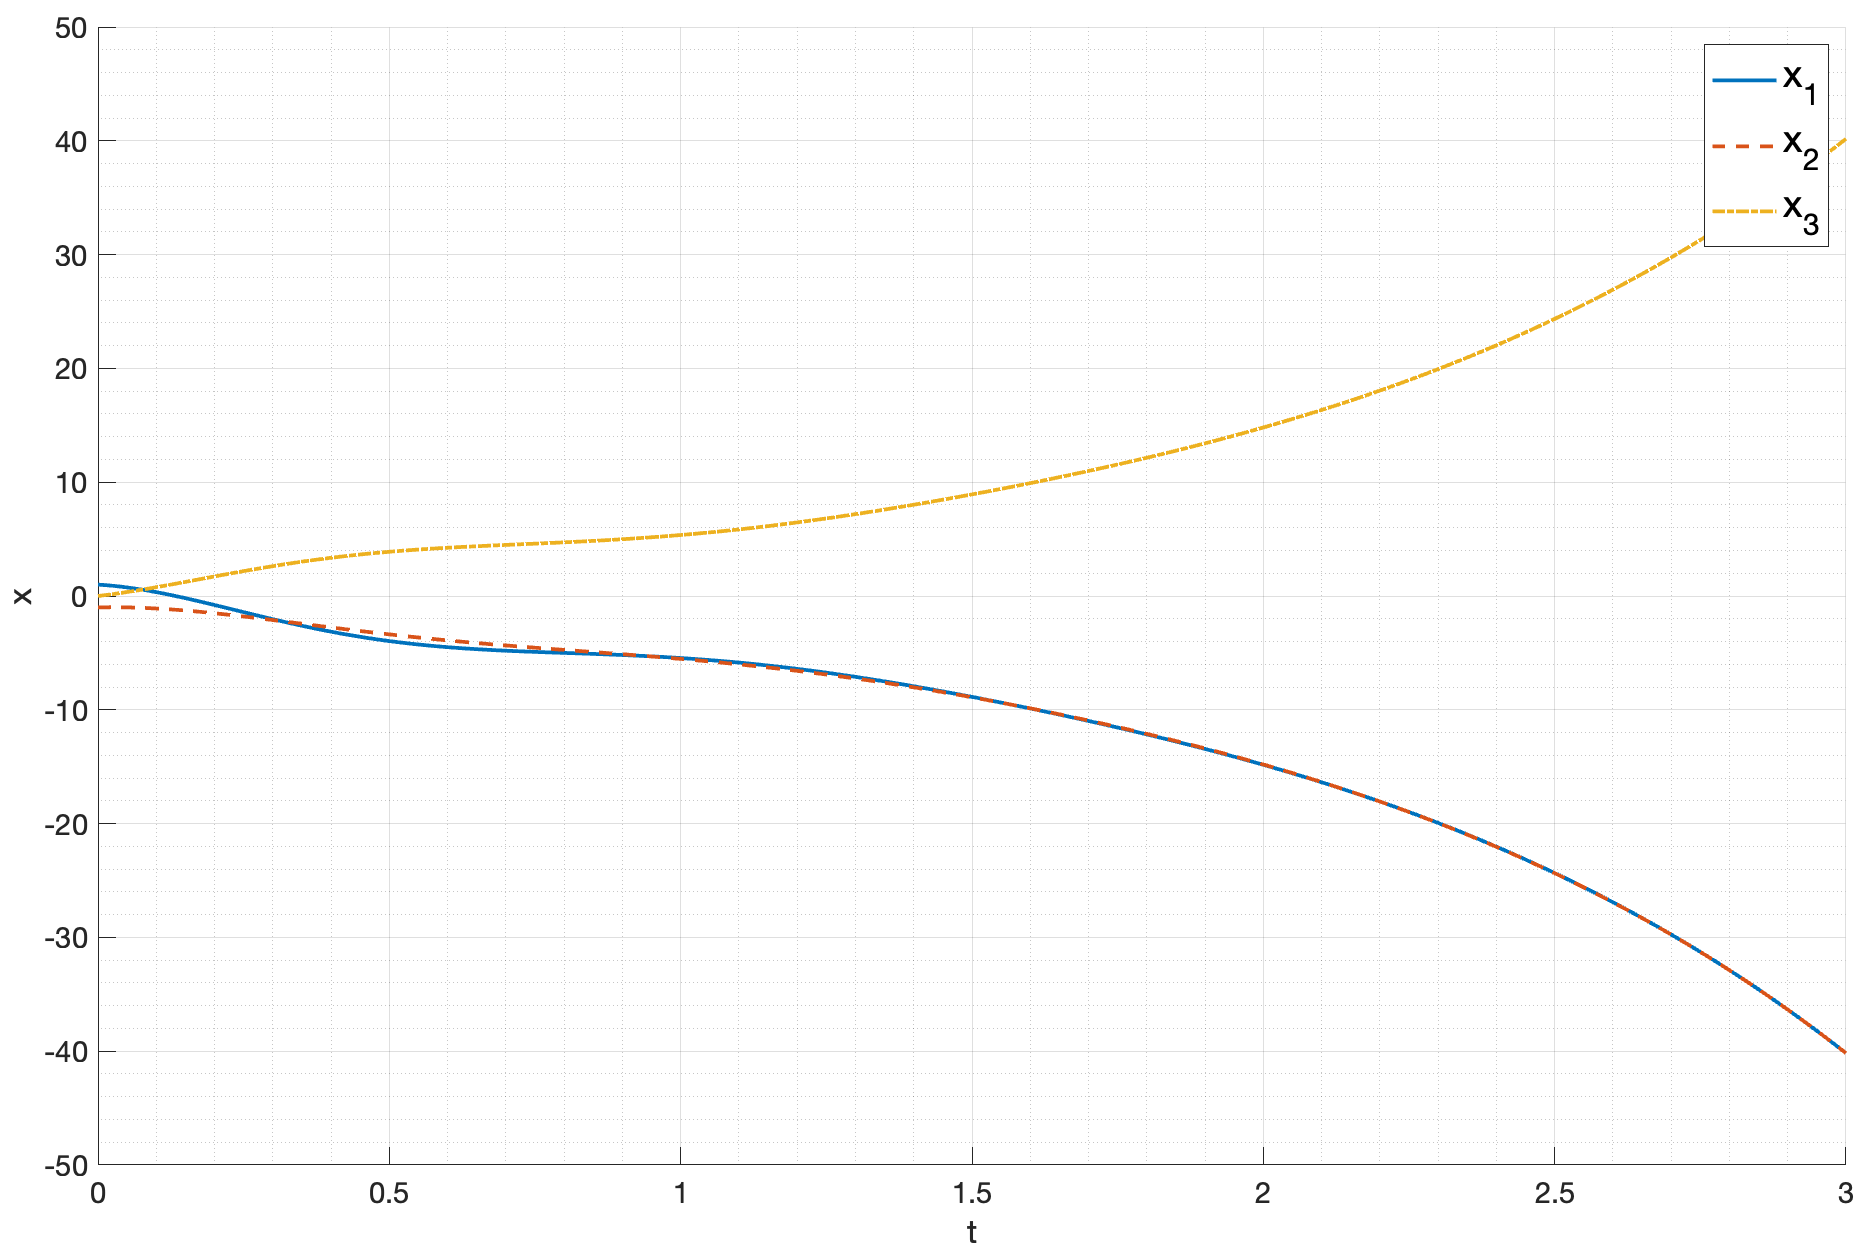
\includegraphics[width=\textwidth]{media/plots/task4_states.png}
    \caption{Состояния системы}
    \label{fig:task4_states}
\end{figure}
На рисунке \ref{fig:task4_states} изображены состояния системы.
\begin{figure}
    \centering
    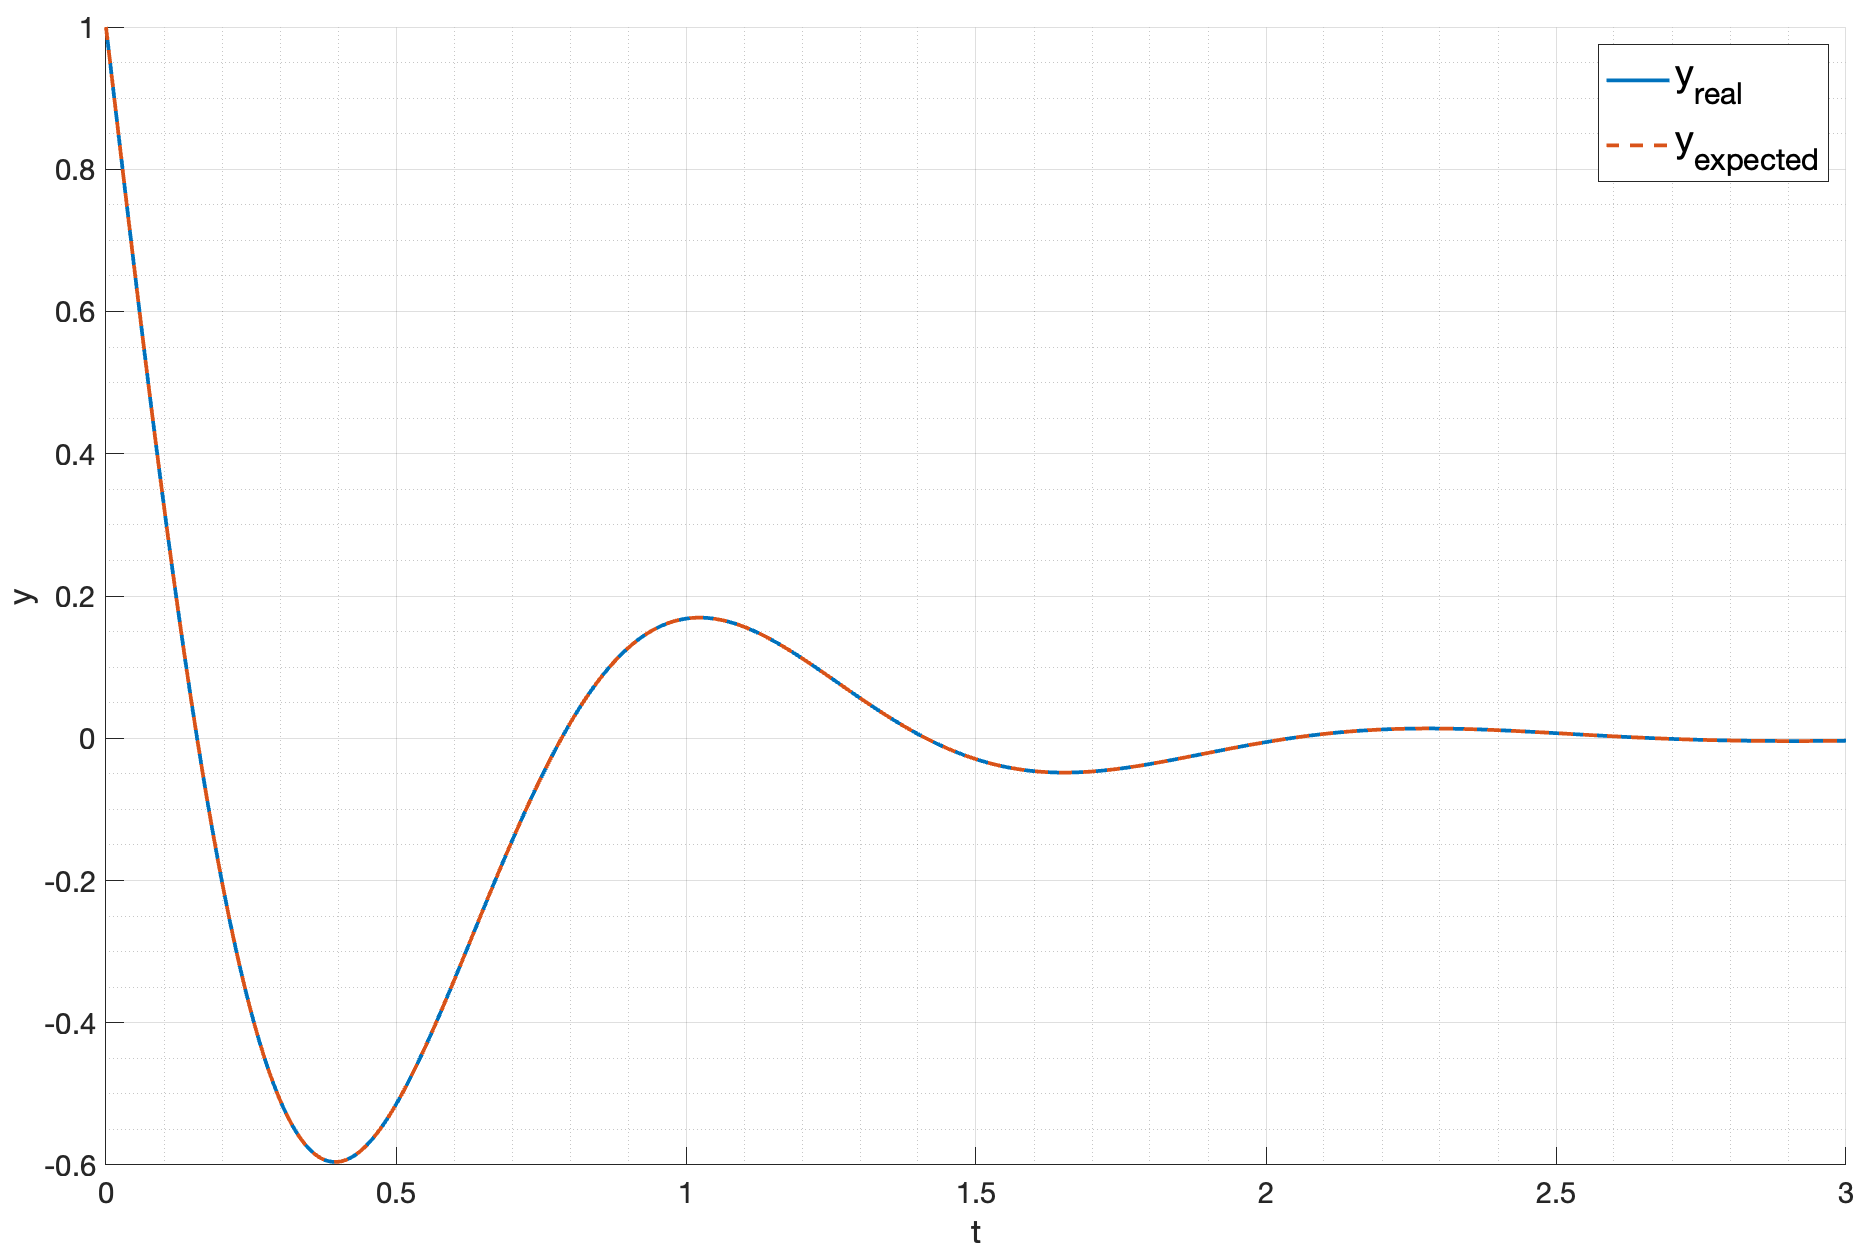
\includegraphics[width=\textwidth]{media/plots/task4_output.png}
    \caption{Выход системы}
    \label{fig:task4_output}
\end{figure}
На рисунке \ref{fig:task4_output} изображен выход системы. Видно, что выход системы совпадает с функцией $y(t)$.
\begin{figure}
    \centering
    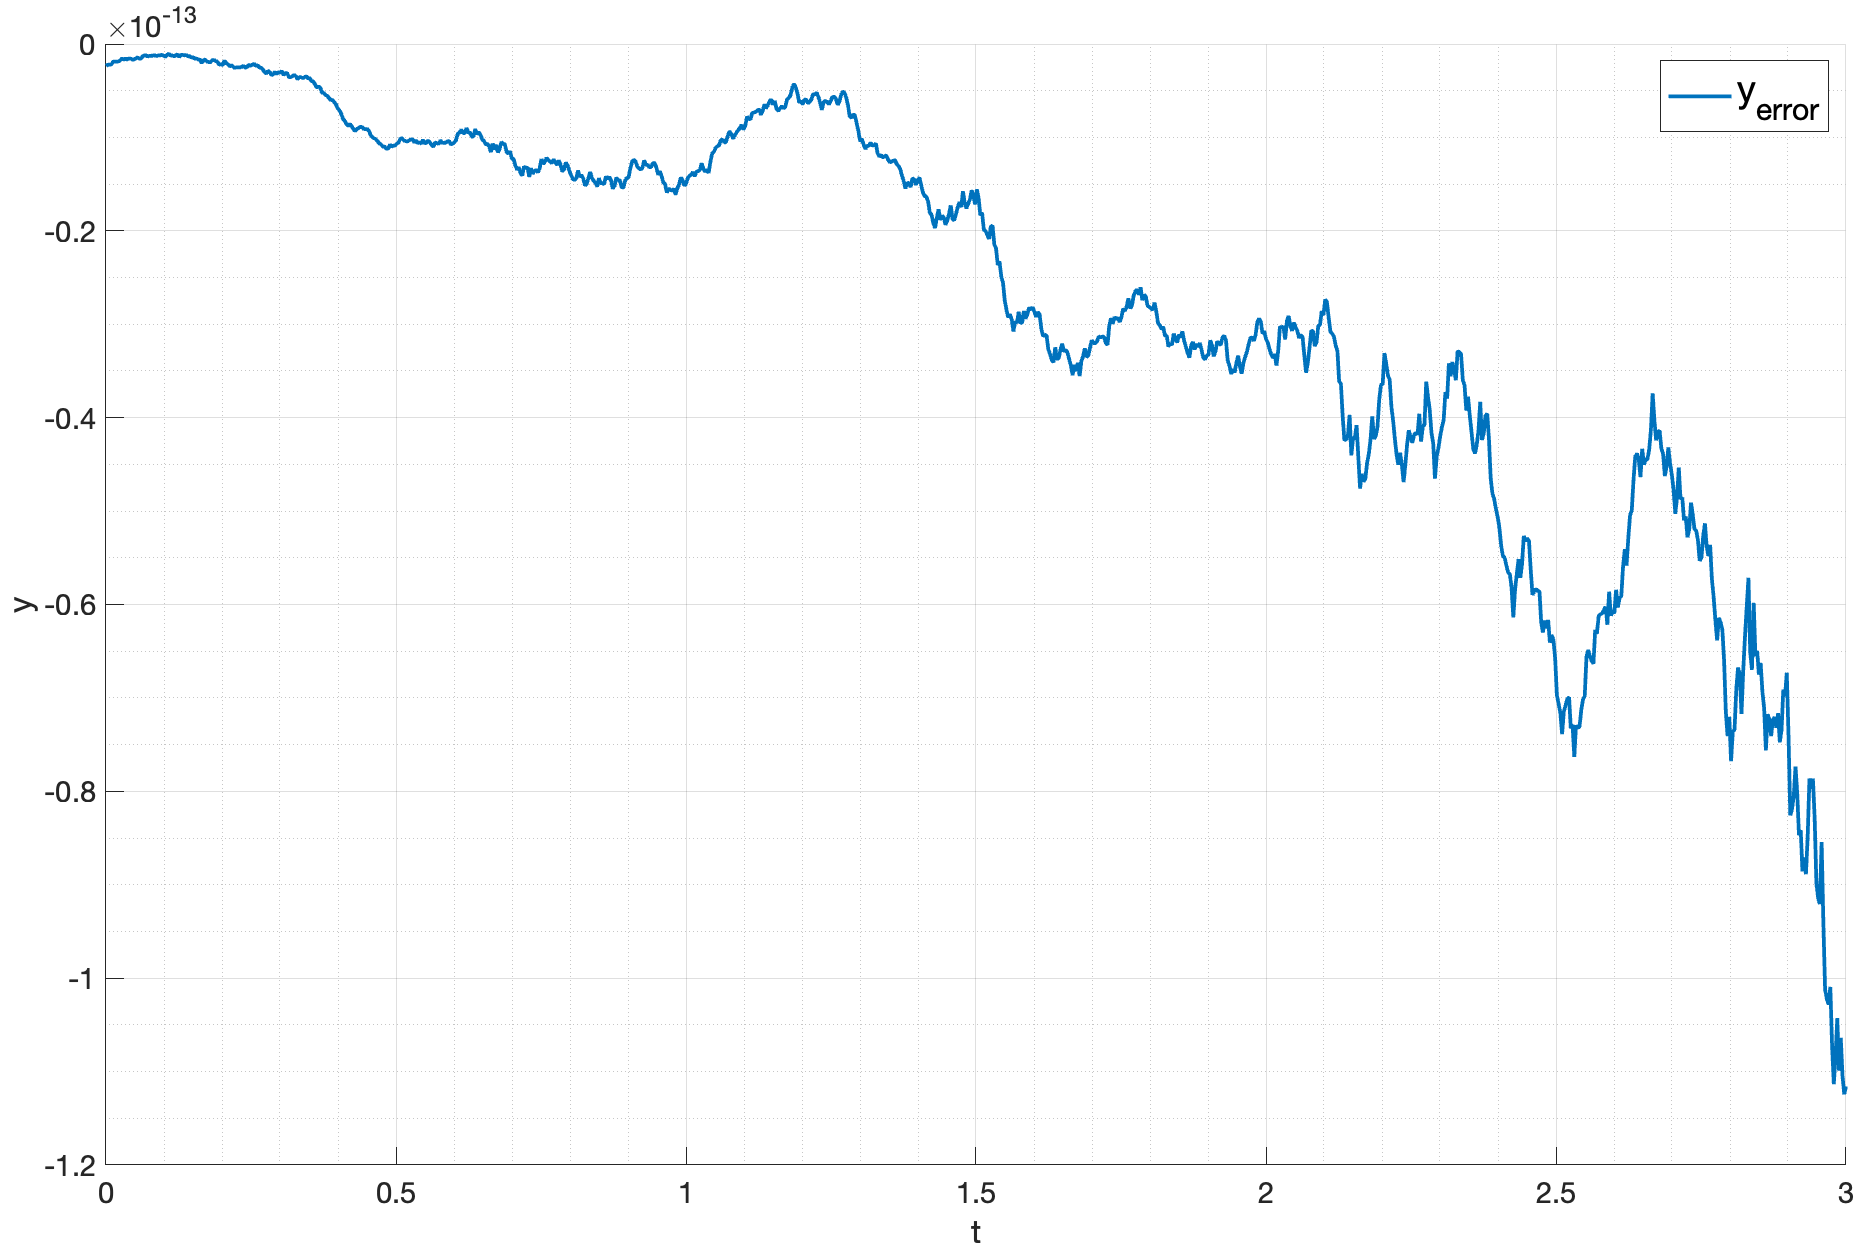
\includegraphics[width=\textwidth]{media/plots/task4_error.png}
    \caption{Ошибка наблюдения}
    \label{fig:task4_estimation}
\end{figure}

\FloatBarrier
\subsection{Альтернативные начальные условия} 
Так как система не является полностью наблюдаемой, то существует бесконечное множество начальных условий,
при которых выход системы совпадает с функцией $y(t)$. Для того, чтобы найти такие начальные условия, необходимо
рассмотреть ядро матрицы наблюдаемости.
\begin{equation}
    \text{Nullspace}(W) =  \text{Nullspace}\left\{\begin{bmatrix}
        -1 \\ -1 \\ 1
    \end{bmatrix}  \right\}
\end{equation}

Таким образом, начальные условия могут быть представлены в виде: 
\begin{equation}
    x(0) = \begin{bmatrix}
        1 \\ -1 \\ 0
    \end{bmatrix} + \alpha \begin{bmatrix}
        -1 \\ -1 \\ 1
    \end{bmatrix}
\end{equation}
где $\alpha \in R$ - произвольное число.

Приведем примеры таких начальных условий:
\begin{equation}
    \begin{array}{cc}
        \hat{x}_1(0) = \begin{bmatrix}
            0 & -2 & 1
        \end{bmatrix}^T, \\
        \hat{x}_2(0) = \begin{bmatrix}
            -19 & -21 & 20
        \end{bmatrix}^T, \\
        \hat{x}_3(0) = \begin{bmatrix}
            -299 & -301 & 300.00 
        \end{bmatrix}^T, \\
        \ldots
    \end{array}
\end{equation}
Проведем моделирование системы с этими начальными условиями: 
\begin{enumerate}
    \item $\hat{x}_1(0) = \begin{bmatrix}
        0 & -2 & 1
    \end{bmatrix}^T$; графики состояний и выхода системы представлены на рисунках \ref{fig:task4_states_hat_1} и \ref{fig:task4_output__hat_1} соответственно.
    \item $\hat{x}_2(0) = \begin{bmatrix}
        -19 & -21 & 20
    \end{bmatrix}^T$; графики состояний и выхода системы представлены на рисунках \ref{fig:task4_states_hat_2} и \ref{fig:task4_output_hat_2} соответственно.
    \item $\hat{x}_3(0) = \begin{bmatrix}
        -299 & -301 & 300 
    \end{bmatrix}^T$; графики состояний и выхода системы представлены на рисунках \ref{fig:task4_states_hat_3} и \ref{fig:task4_output__hat_3} соответственно.
\end{enumerate}

\begin{figure}[ht!]
    \centering
    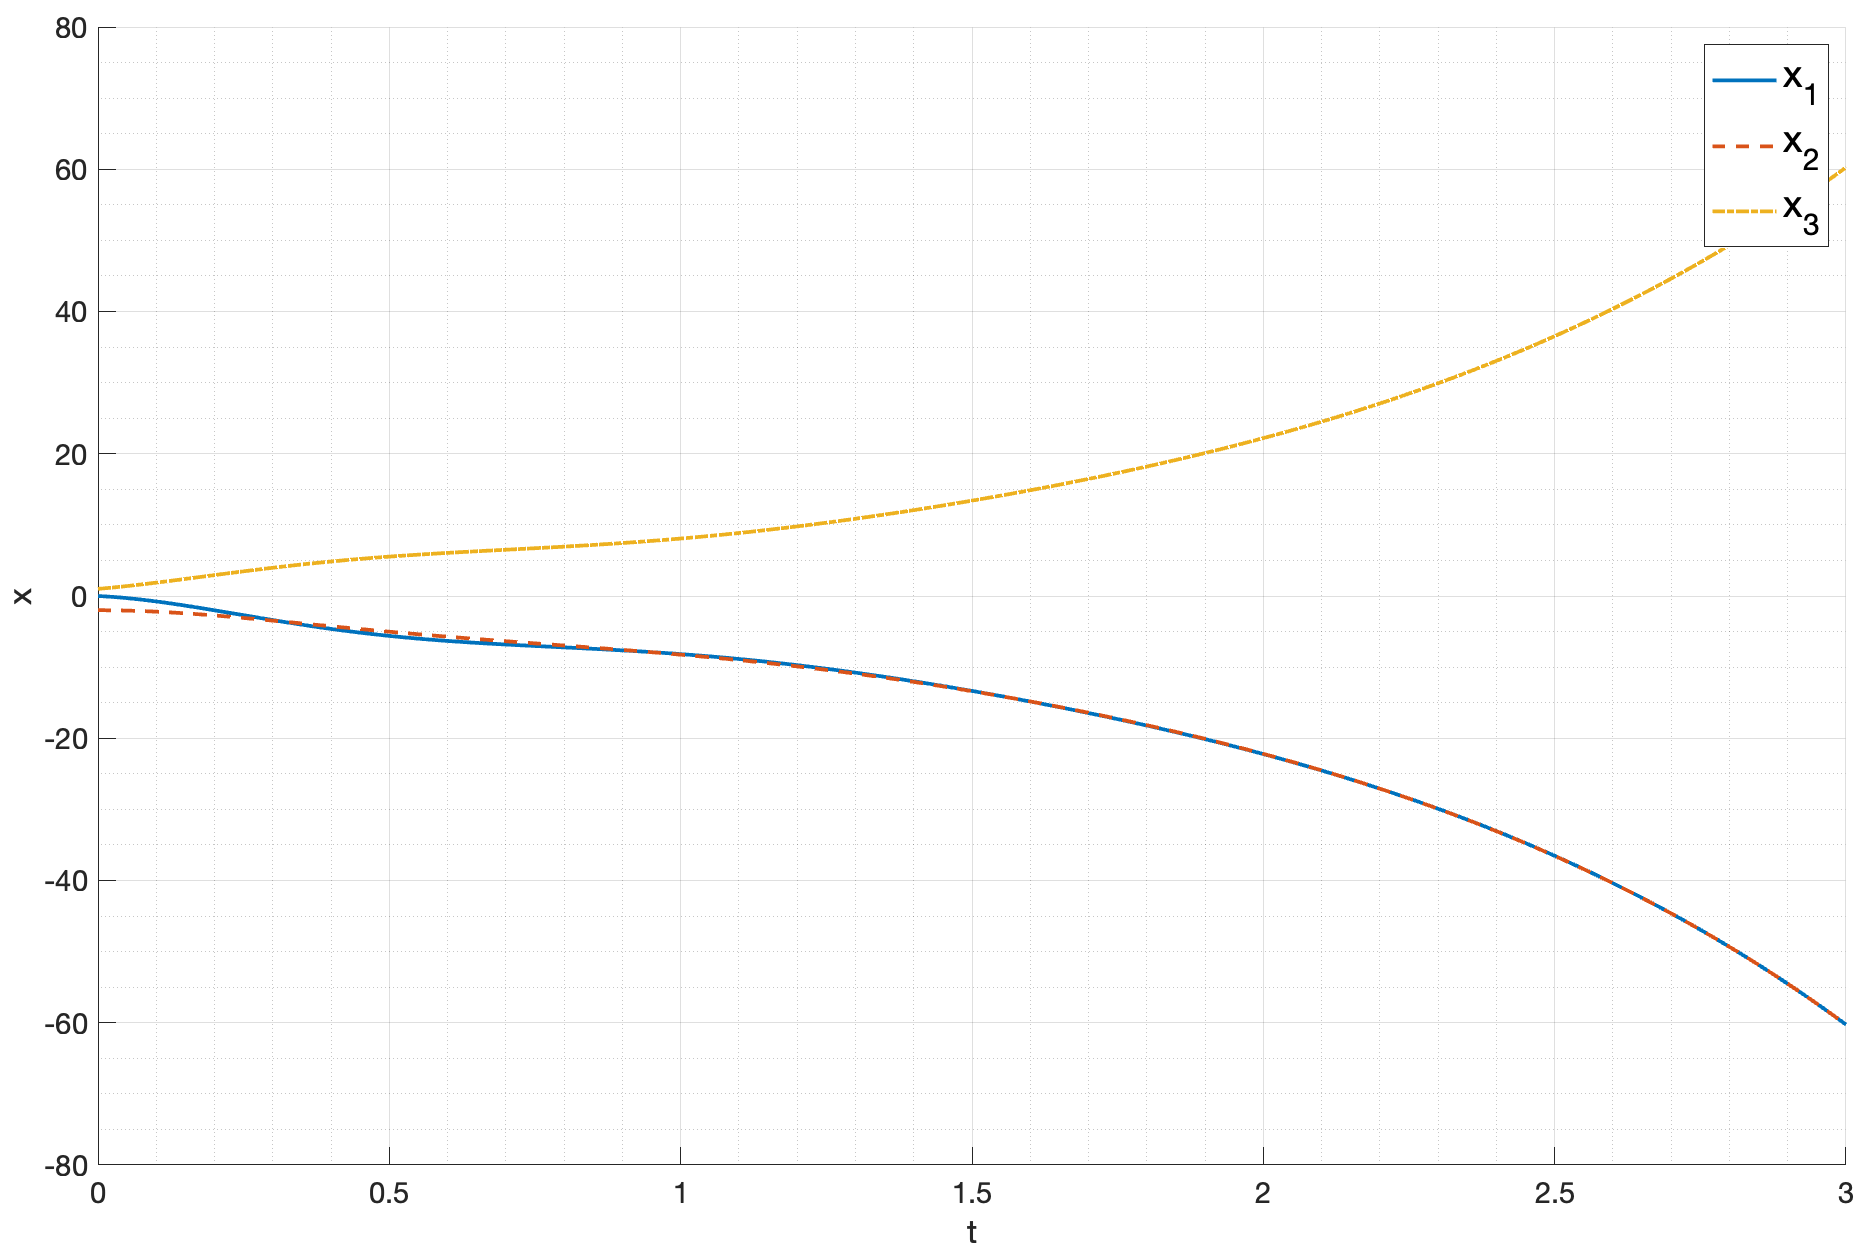
\includegraphics[width=\textwidth]{media/plots/task4_states_hat_1.png}
    \caption{Состояния системы с начальными условиями $\hat{x}_1(0)$}
    \label{fig:task4_states_hat_1}
\end{figure}

\begin{figure}[ht!]
    \centering
    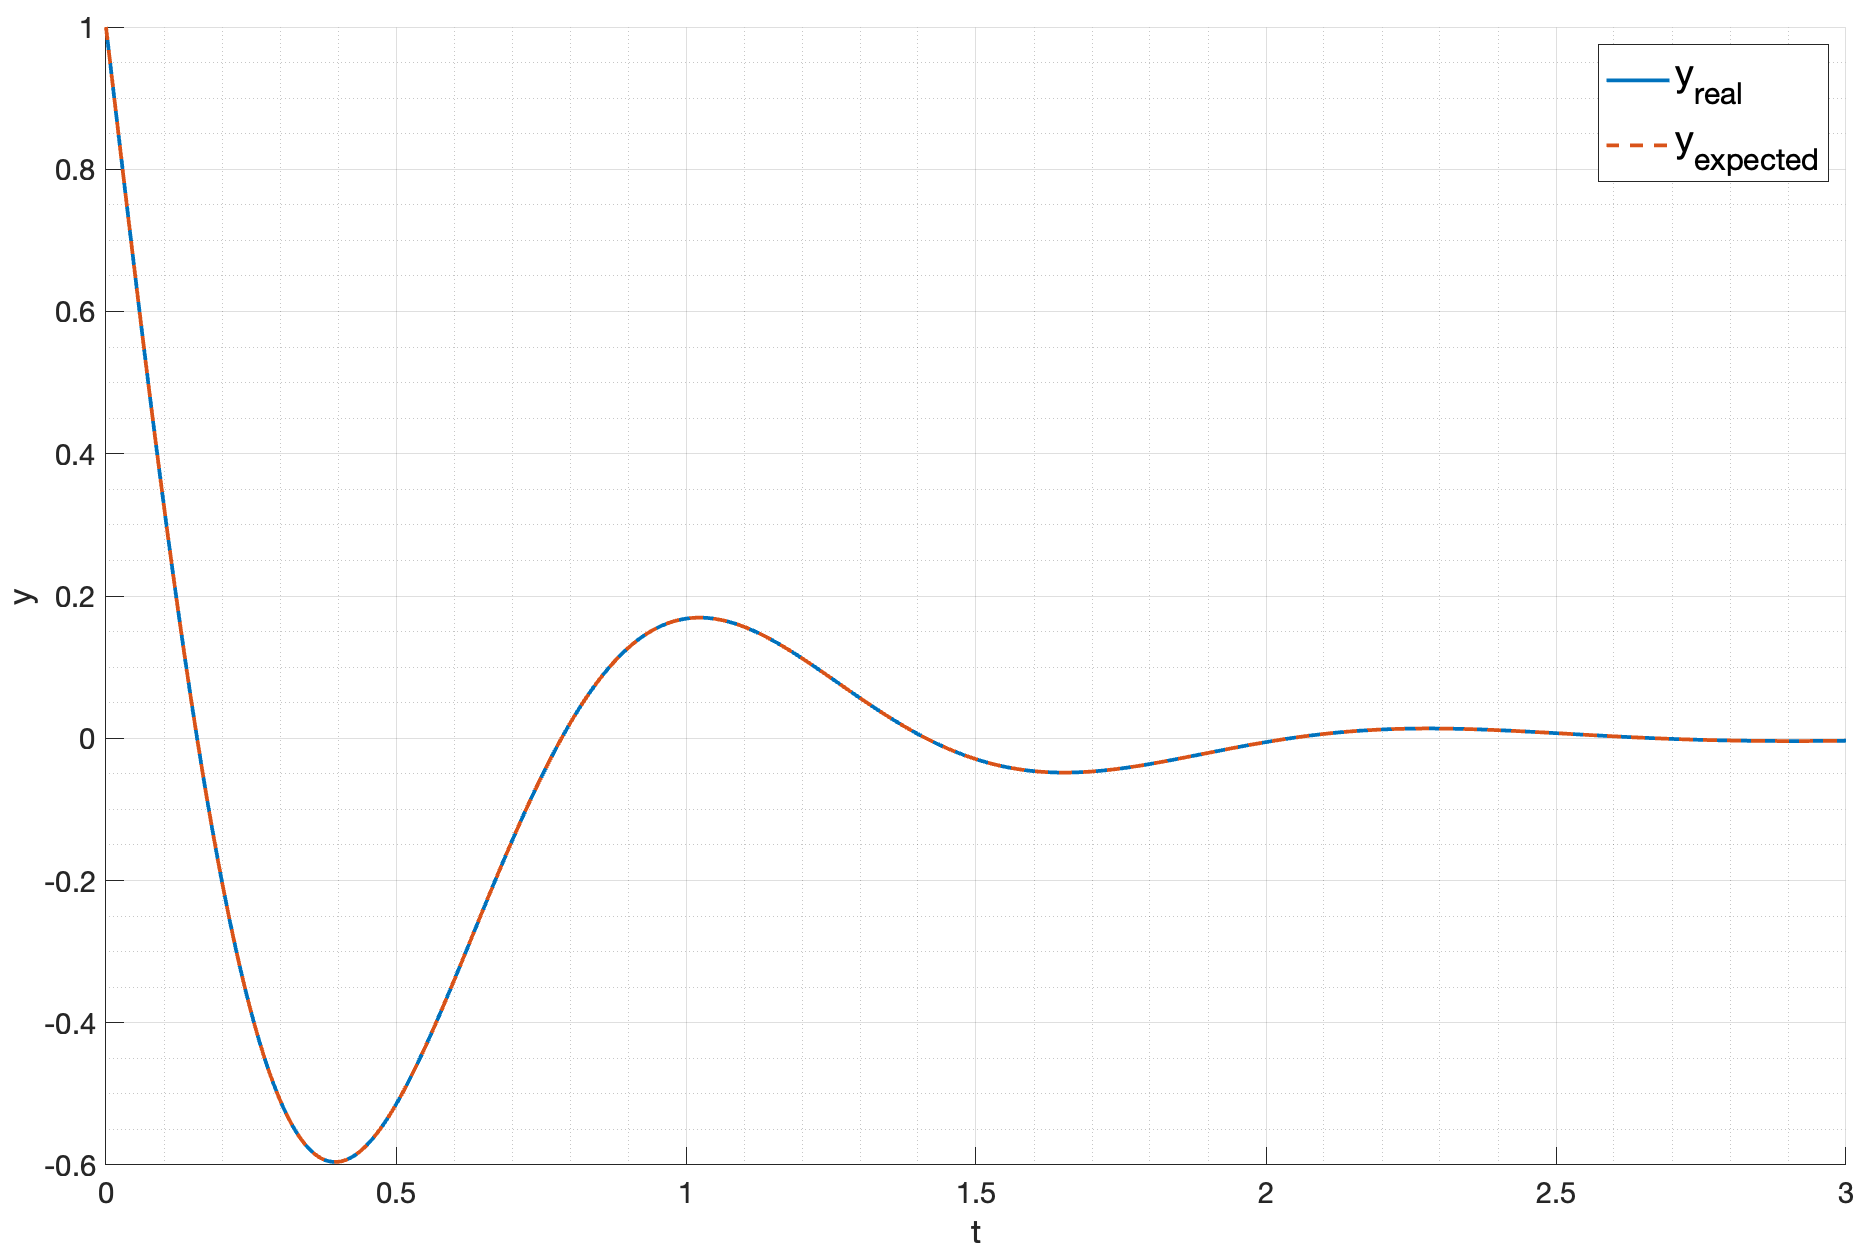
\includegraphics[width=\textwidth]{media/plots/task4_output_hat_1.png}
    \caption{Выход системы с начальными условиями $\hat{x}_1(0)$}
    \label{fig:task4_output__hat_1}
\end{figure}

\begin{figure}[ht!]
    \centering
    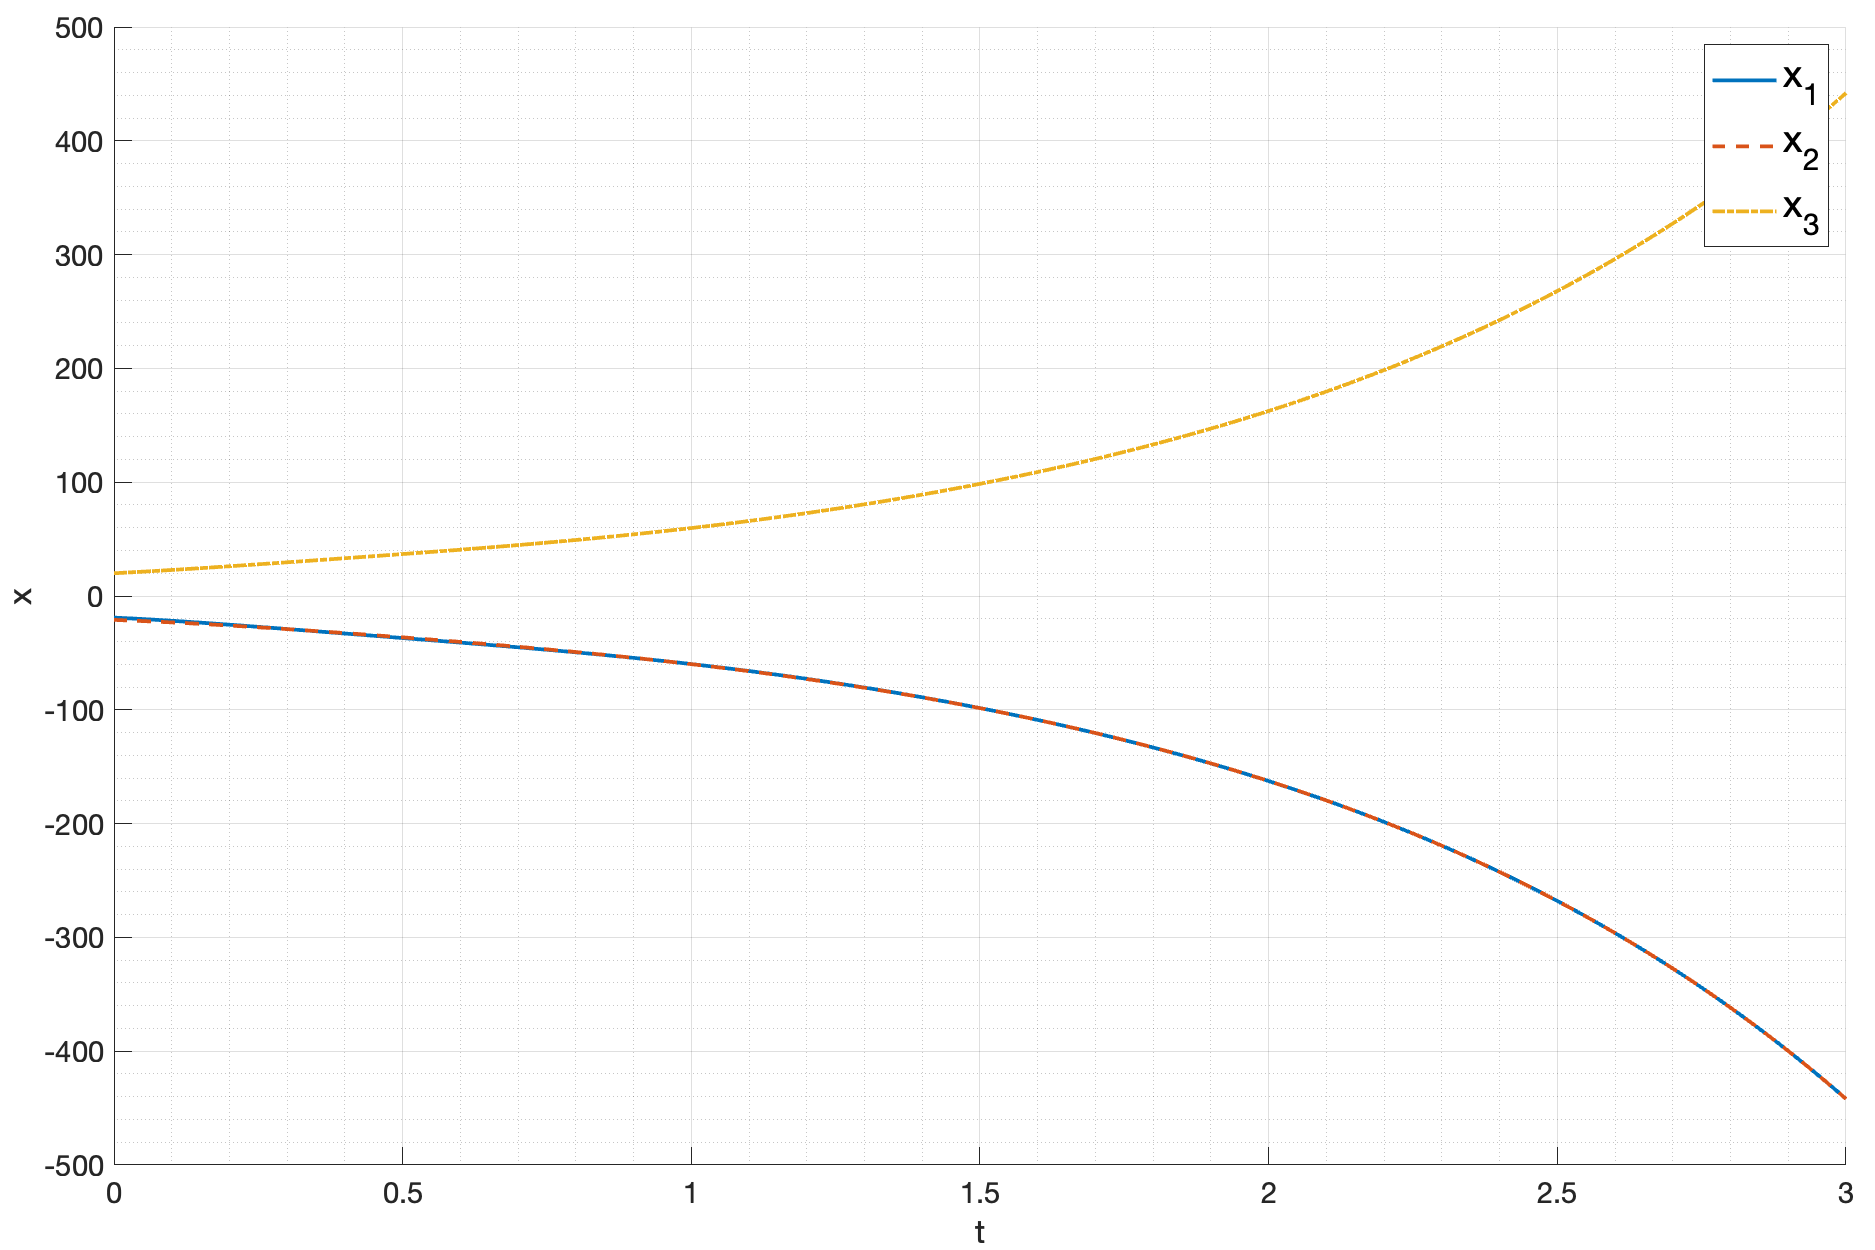
\includegraphics[width=\textwidth]{media/plots/task4_states_hat_2.png}
    \caption{Состояния системы с начальными условиями $\hat{x}_2(0)$}
    \label{fig:task4_states_hat_2}
\end{figure}

\begin{figure}[ht!]
    \centering
    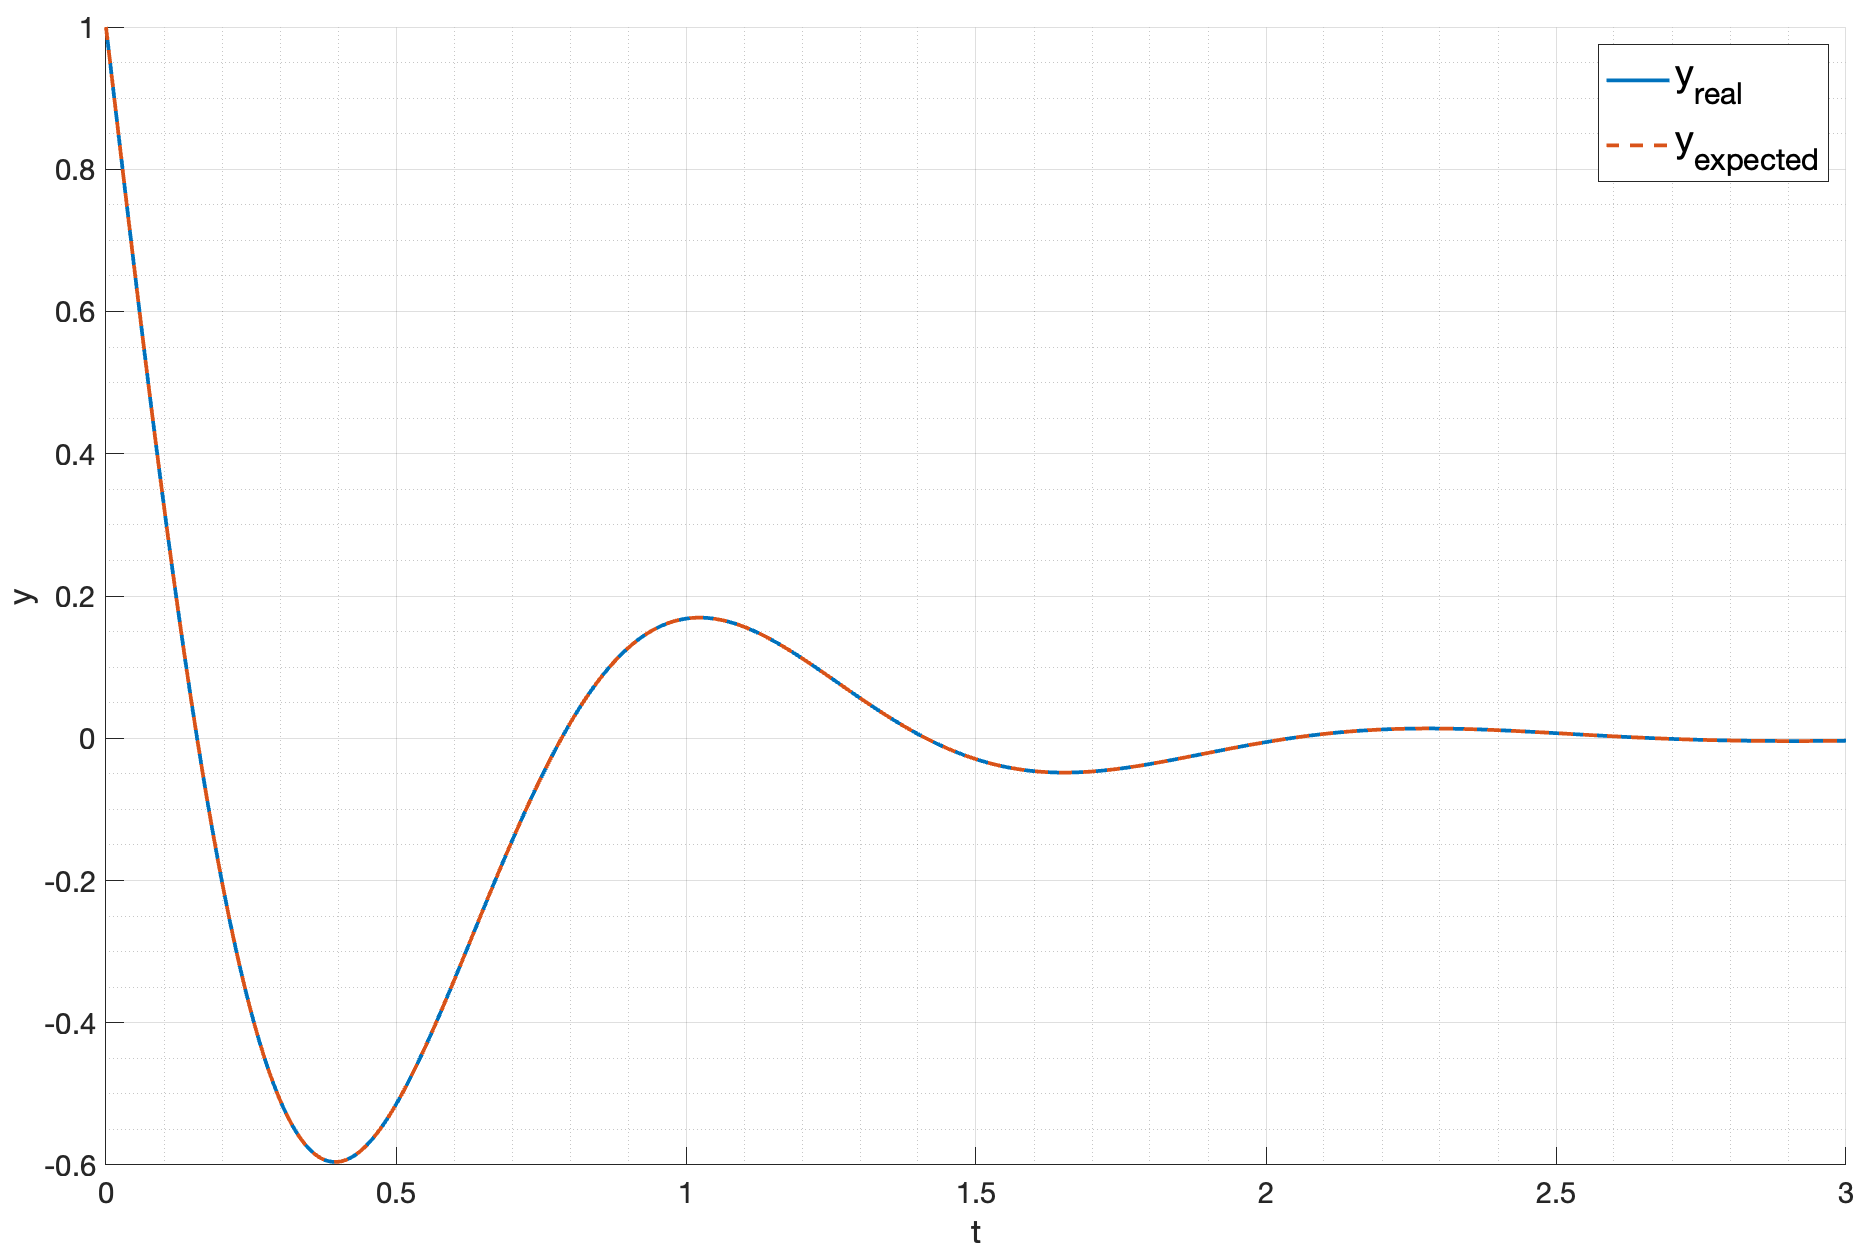
\includegraphics[width=\textwidth]{media/plots/task4_output_hat_2.png}
    \caption{Выход системы с начальными условиями $\hat{x}_2(0)$}
    \label{fig:task4_output_hat_2}
\end{figure}

\begin{figure}[ht!]
    \centering
    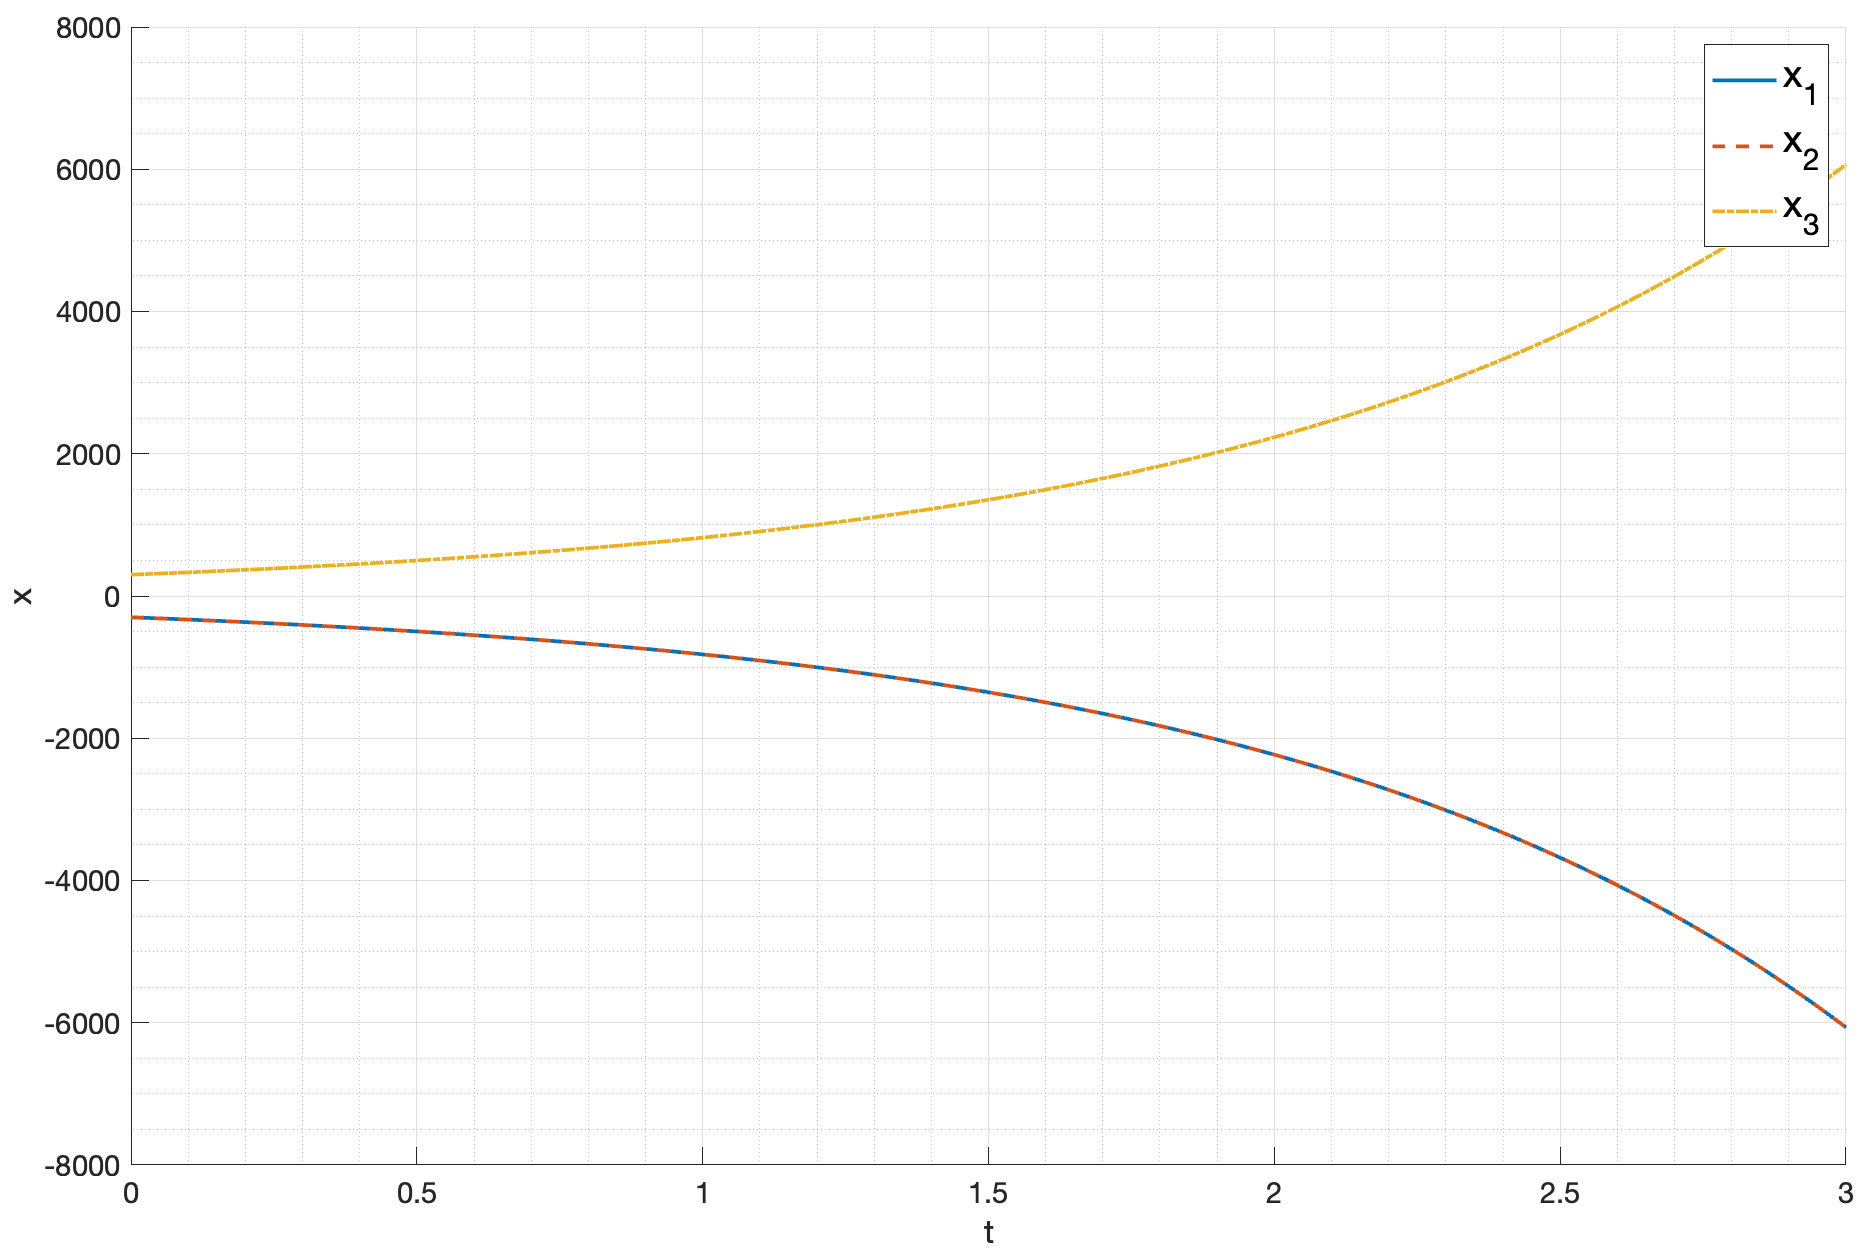
\includegraphics[width=\textwidth]{media/plots/task4_states_hat_3.png}
    \caption{Состояния системы с начальными условиями $\hat{x}_3(0)$}
    \label{fig:task4_states_hat_3}
\end{figure}

\begin{figure}[ht!]
    \centering
    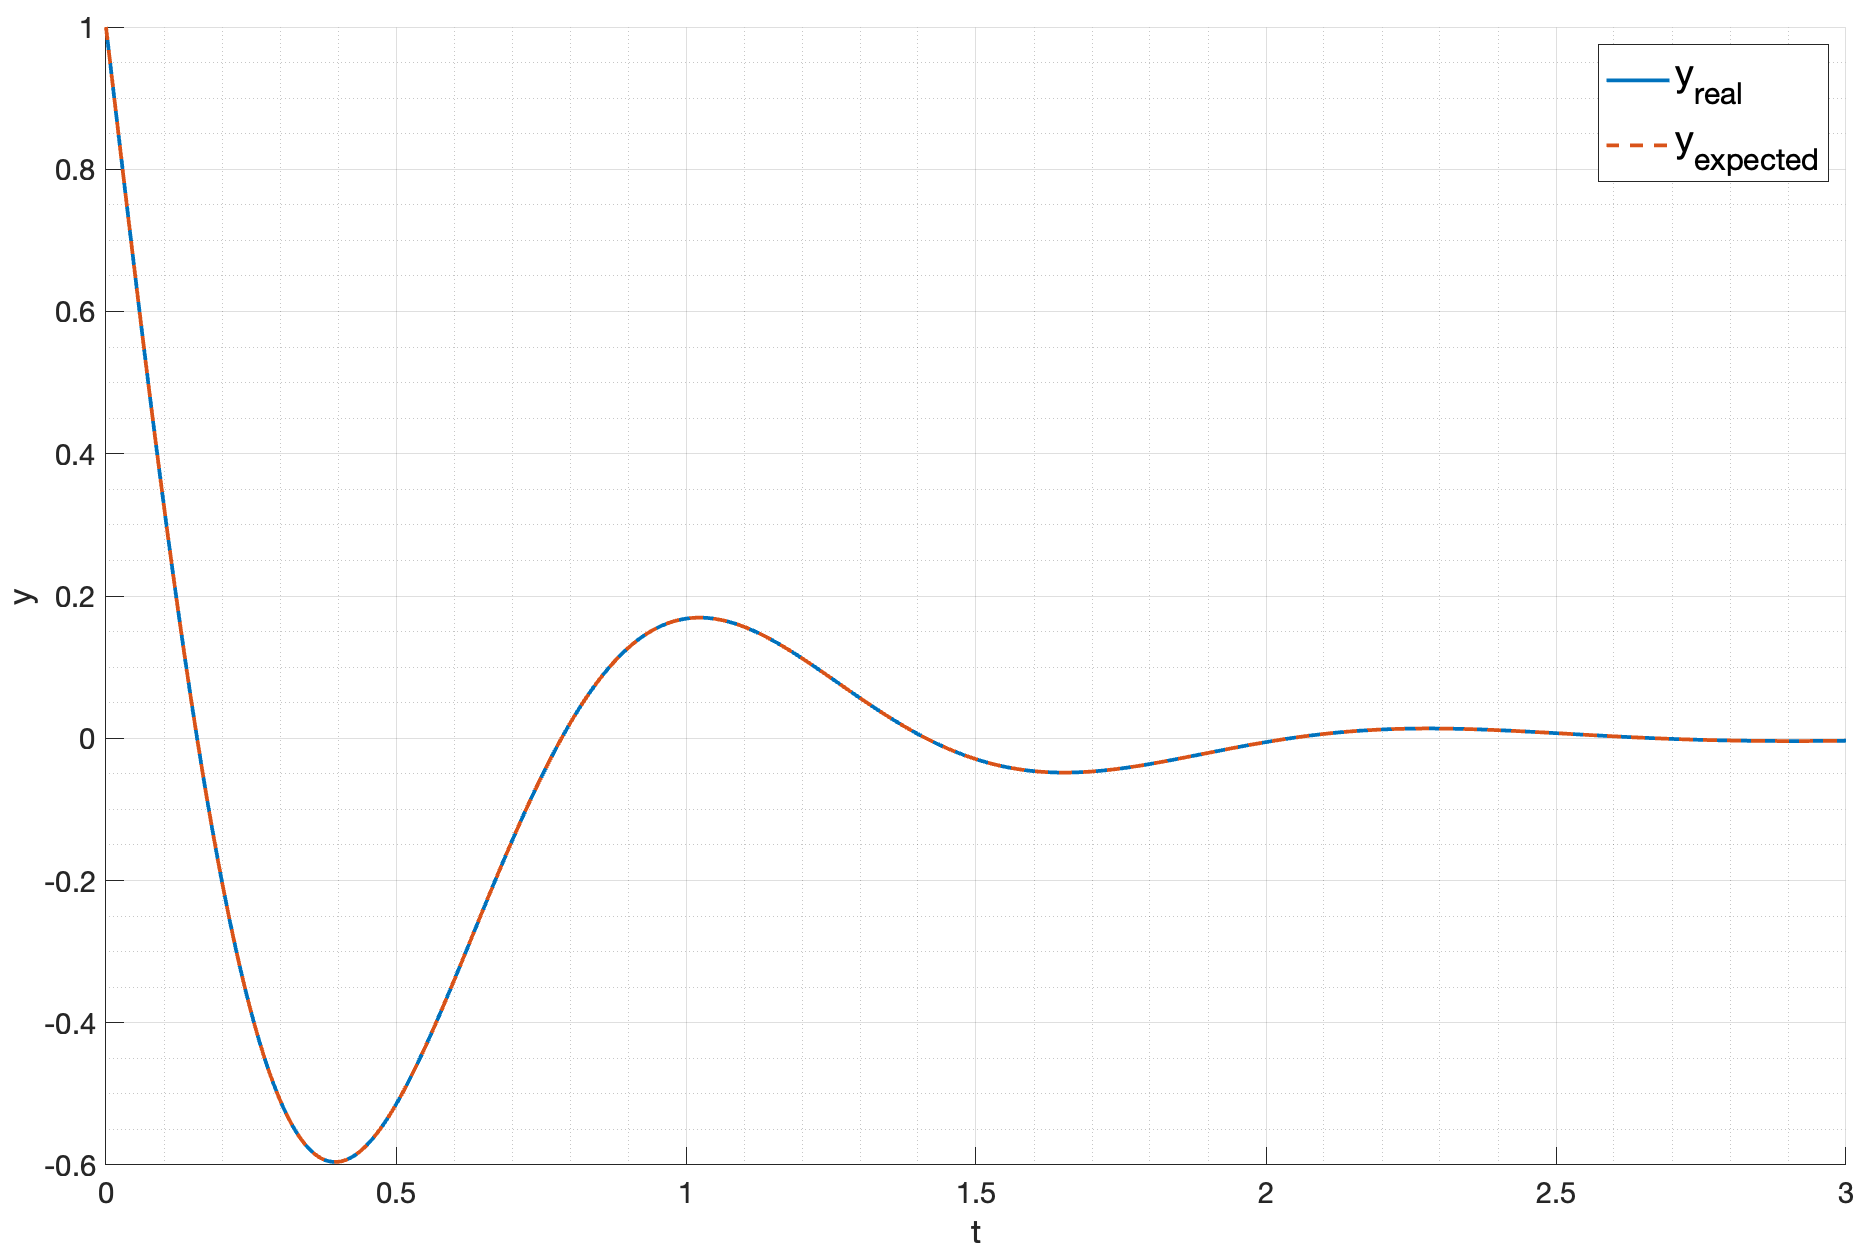
\includegraphics[width=\textwidth]{media/plots/task4_output_hat_3.png}
    \caption{Выход системы с начальными условиями $\hat{x}_3(0)$}
    \label{fig:task4_output__hat_3}
\end{figure}

Видно, что при всех этих начальных условиях выход системы совпадает с функцией $y(t)$.

\subsection{Вывод}
При исследовании системы, рассматриваемой в этом задании, удалось показать, что она не является полностью наблюдаемой.
Это было продемонстрировано с помощью критерия Калмана, через наблюдаемость собственных значений и диагональную форму системы. 
Также был найден грамиан наблюдаемости и проверены его собственные числа. 
Проведено моделирование системы с различными начальными условиями, при которых выход системы совпадает с заданной функцией. 
Результаты моделирования показали, что система не является полностью наблюдаемой, то есть 
невозможно однозначно восстановить начальные условия системы по ее выходу.